\documentclass[12pt, a4paper]{article}

% ---- packages -----------------------------------------------
\usepackage[utf8]{inputenc}
\usepackage[T1]{fontenc}
\usepackage{geometry}
\geometry{margin=0.75in}
\usepackage{graphicx}
\usepackage{booktabs}
\usepackage{amsmath}
\usepackage{amssymb}
\usepackage{array}
\usepackage[round]{natbib}
\usepackage[hidelinks]{hyperref}
\usepackage{float}
\usepackage{caption}
\usepackage{subcaption}
\usepackage{parskip}
\usepackage{microtype}
\usepackage{xcolor}
\usepackage[nosep]{enumitem}
\usepackage[compact]{titlesec}
\usepackage{multirow}
\titleformat{\section}{\large\bfseries}{\thesection}{1em}{}
\titleformat{\subsection}{\normalsize\bfseries}{\thesubsection}{1em}{}
\titleformat{\subsubsection}{\normalsize\itshape}{\thesubsubsection}{1em}{}
\setlength{\textfloatsep}{8pt plus 1.0pt minus 2.0pt}
\setlength{\intextsep}{8pt plus 1.0pt minus 2.0pt}
\setlength{\floatsep}{8pt plus 1.0pt minus 2.0pt}
\linespread{1.10}

\begin{document}

% ============================================================
%  TITLE
% ============================================================
\begin{center}
  \vspace*{-2em}
  {\Large \textbf{Report 2: Sentence Memorability Experiment}}\\[6pt]
  {\normalsize \textbf{Idle Death Gamblers}}\\[2pt]
  {\small Shreyas Deb \quad Yajat Lakhanpal \quad Prasoon Dev}\\[4pt]
  {\small \textit{BRSM Project --- SP 2026}}
\end{center}
\vspace{0.3em}

% ============================================================
\section{Introduction}
% ============================================================

\subsection{Sentence Memory: Gist vs.\ Wording}

Human memory for language is not a faithful archive of words and syntax.
A central finding in cognitive psychology is that listeners and readers
retain the \emph{meaning} (gist) of sentences with much greater fidelity
than their verbatim wording or grammatical structure. The
\emph{kernel-plus-tag} hypothesis \citep{miller1962,mehler1963} proposed
that sentences are encoded as a semantic kernel with syntactic features
stored as forgettable tags. \citet{bregman1968} refuted this: when
participants misidentified the syntactic form on a first guess, their
second guesses exceeded chance ($\chi^2(4) = 20.8$, $p < .001$),
suggesting that grammatical form is \emph{reconstructed} from imagery and
noun salience rather than retrieved as a tag.

\citet{begg1971} tested the gist--wording dissociation directly via a
\textbf{continuous recognition paradigm}. Meaning judgments declined
sharply with lag ($r = -.996$), while wording judgments were uncorrelated
with lag ($r = -.107$), interpreted as evidence that concrete sentence
meaning is stored as a spatial image and wording is reconstructed from
that image trace at retrieval.

If wording is reconstructed from an imagistic trace, the imageability of
constituent nouns becomes critical. \citet{james1973} tested this in free
recall using four noun-imageability conditions (HH, HL, LH, LL) and
documented a threshold-like recall pattern and a bias toward placing
salient nouns in subject position during reconstruction.

% ------------------------------------------------------------
\subsection{Signal Detection Theory Motivation}
\label{sec:sdt_lit}

In recognition-memory tasks, raw accuracy or corrected hit-minus-false-alarm
scores can obscure an important distinction between two processes: how well
participants discriminate old from new items, and how conservatively they
choose to respond ``old.'' Signal Detection Theory (SDT;\,\citealt{green1966})
addresses this by separating \textbf{sensitivity} ($d'$) from
\textbf{response criterion} ($c$), and has long been the standard framework
for recognition-memory research \citep{macmillan2005}. We therefore use SDT
as a downstream analysis to test whether the observed noun-condition
differences reflect a genuine change in discriminability ($d'$) or instead
arise from shifts in response bias ($c$). The non-parametric index $A'$
\citep{snodgrass1988} is included as a robustness measure that requires no
Gaussian equal-variance assumption.

% ------------------------------------------------------------
\subsection{Core Question and Hypotheses}

Recognition memory presents participants with an item and asks ``have
you seen this before?'' (a discrimination judgment), whereas free recall
requires generating studied items from scratch. Recognition is generally
more sensitive to weak memory traces --- a property that is theoretically
important here, as it may explain why a \emph{single} high-imageability
noun suffices to anchor a recognition decision (threshold pattern) while
free recall shows a more graded benefit \citep{james1973}.

The present study extends \citet{james1973} from free recall to online
continuous recognition, tests \citet{begg1971}'s prediction that
imageability selectively affects gist but not wording, and uses SDT to
decompose the imageability effect into sensitivity and criterion components.

\begin{enumerate}[label=\textbf{H\arabic*:}]
  \item \textbf{(Gist):} Corrected IR differs across noun imageability
  conditions (HH, HL, LH, LL), with LL showing the largest deficit.
  \item \textbf{(Wording):} WR accuracy is not significantly affected by
  noun imageability; voice is reconstructed from the imagistic trace.
  \item \textbf{(Voice):} Active-voice sentences will show different
  memorability and wording-recognition patterns compared to passive.
  \item \textbf{(No Interaction):} Voice does not moderate the noun
  imageability effect on Corrected IR or WR.
\end{enumerate}

% ============================================================
\section{Dataset and Experimental Design}
% ============================================================

\subsection{Participants}

Data were collected from 114 online participants. Two participants failed
the vigilance criterion on all three blocks and were excluded, leaving
\textbf{112 participants} (block pass rate: 96.2\%, 329/342 blocks).

\subsection{Design}

Fully within-participants \textbf{4 (Noun Condition: HH, HL, LH, LL)
$\times$ 2 (Voice: Active, Passive)} design. Noun conditions were defined
by crossing subject and object noun imageability (Table~\ref{tab:conditions}).
High-Frequency (HF) filler sentences served as lures for false alarm
estimation.

\begin{table}[htbp]
  \centering\small
  \begin{tabular}{lll}
    \toprule
    \textbf{Code} & \textbf{Subject Noun} & \textbf{Object Noun} \\
    \midrule
    HH & High imageability & High imageability \\
    HL & High imageability & Low imageability  \\
    LH & Low imageability  & High imageability \\
    LL & Low imageability  & Low imageability  \\
    \bottomrule
  \end{tabular}
  \caption{Four experimental noun conditions.}
  \label{tab:conditions}
\end{table}

\subsection{Stimuli}

Simple SVO sentences were constructed by crossing noun imageability
levels with voice. High- and low-imageability nouns were selected using
the concreteness and imagery norms of \citet{paivio1968}; verbs were
medium-concreteness action verbs. After fluency and coherence filters,
200 active-voice sentences (50 per condition) were selected and each
converted to passive, yielding \textbf{400 target sentences} plus HF
lure sentences.

\subsection{Procedure}

Participants completed a continuous recognition task across
\textbf{3 experimental blocks} preceded by a practice block. Each
sentence was displayed for $\approx$4000~ms (ITI: 700--1300~ms). For
each probe, participants made two sequential judgments:
\begin{enumerate}[nosep]
  \item \textbf{IR:} ``Have you seen this sentence before?'' (spacebar).
  \item \textbf{WR:} ``Same grammatical voice?'' (key press; elicited
  only when IR was pressed).
\end{enumerate}

\subsection{Validation and Exclusions}

Raw event logs (81,329 rows) were processed in R. Block boundaries were
identified from ``Rest Phase started'' markers; per-trial accuracy
variables were extracted from \texttt{IR pressed} and \texttt{WR pressed}
rows. Each block was retained only if:
\[
  \text{Correct Validation IRs} >
  \tfrac{\text{Wrong Validation IRs}}{2} + \text{Missed Validation IRs}
\]
Failed blocks were excluded; two participants failing all blocks were
removed entirely, leaving 48,281 observations. The design was balanced:
each noun condition contributed 1,316 encoding trials; each voice
condition 2,632 trials.

\textbf{Practice block exclusion.} Practice blocks were excluded from all
inferential analyses because they were designed only to familiarise
participants with the response interface, not to measure stable
sentence-memory performance. Including them would introduce variance due
to interface acclimatisation (learning key assignments, calibrating
response pacing) that is unrelated to noun imageability processing.
The block-learning analysis tests changes across the three
\emph{experimental} blocks; this question is only answerable cleanly
if every observation reflects fully-familiarised participants responding
to proper experimental stimuli.

% ============================================================
\section{Methods}
% ============================================================

\subsection{Scoring}

False alarm counts were computed from \texttt{IR pressed} events on HF
first-showing trials:
\[
  \widehat{\text{FA rate}} = \frac{\text{IR presses on HF first-showings}}
                                  {\text{HF first-showing display events}}
  \quad (M = 0.160,\; SD = 0.104,\; \text{range: } 0.00\text{--}0.43)
\]

Three dependent variables were derived per participant per cell:
\begin{enumerate}[nosep]
  \item \textbf{Corrected IR:} $\text{IR}_{CR} = \text{Hit Rate} - \text{FA Rate}$.
  \item \textbf{WR Accuracy:} Proportion of correct voice judgments,
  conditional on IR pressed.
  \item \textbf{IR Reaction Time (RT):} Mean RT on correct target probes.
\end{enumerate}

\subsection{Primary Non-Parametric Analysis}

Shapiro-Wilk tests per condition group confirmed that Corrected IR and
WR Accuracy are non-normal in all four groups ($p < .001$), expected
given that these are bounded proportions computed from 3--6 trials per
cell. Non-normality justifies \textbf{Friedman's test} as the omnibus
statistic. Friedman's is the within-participants equivalent of
Kruskal-Wallis: it blocks on participant identity, ranks observations
within each participant, and tests for systematic rank differences across
conditions without distributional assumptions.

Three omnibus Friedman tests (IR CR, WR Accuracy, IR RT) require a
Bonferroni correction: $\alpha_{\text{FW}} = 0.05/3 = .0167$. Within
significant omnibus tests, Holm-corrected paired Wilcoxon signed-rank
post-hoc tests were conducted. Noun condition $\times$ voice interactions
were evaluated with \textbf{Scheirer-Ray-Hare (SRH) tests} (the
non-parametric two-way analogue of ANOVA; cell balance confirmed,
$N = 112$ per cell). SRH was designed for independent groups; sensitivity
Friedman tests per voice level follow as a robustness check.

\subsection{SDT Analysis}

\textbf{Rationale.} The corrected IR score is useful as a bias-reduced
behavioural summary but does not fully separate memory strength from
response strategy. SDT provides that decomposition by estimating
sensitivity ($d'$) and criterion ($c$) from hit and false-alarm rates
\citep{stanislaw1999,macmillan2005}. This allows us to test whether the
LL deficit reflects weaker memory evidence, a more conservative response
threshold, or both.

SDT parameters were computed per participant per noun condition using
log-linear correction (adding 0.5 to counts, 1 to denominators) to
prevent infinite $z$-values \citep{macmillan2005}. The non-parametric
$A'$ index \citep{snodgrass1988}:
\[
  A' = 0.5 + \frac{(\text{HR} - \text{FAR})(1 + \text{HR} - \text{FAR})}
                   {4 \cdot \text{HR} \cdot (1 - \text{FAR})}
  \quad (\text{when HR} \geq \text{FAR})
\]
is bounded in $[0.5,1]$ and requires no equal-variance assumption,
serving as an independent check on $d'$ conclusions. Because $d'$ and $c$
are theoretically unbounded $z$-score transforms and passed Shapiro-Wilk
normality per group ($p > .09$), \textbf{repeated-measures ANOVA} was
used for those indices (in contrast to the non-parametric Friedman tests
applied to bounded proportions); $A'$ uses Friedman's. Convergent
validity was checked via Spearman $\rho(d', \text{Corrected IR})$.

\textbf{Caveat:} All HF lures are active-voice; a global FA rate is
therefore used for both voice conditions, which may marginally inflate
$d'$ for passive sentences. Voice SDT comparisons are interpreted with
this limitation in mind.

\subsection{GLM Analysis}

GLMs were fit at cell level (one row per participant $\times$ noun
condition $\times$ voice; $N = 890$ after listwise exclusion of 6 rows
with no WR trials). Reference levels: noun condition = LL, voice =
Active. Table~\ref{tab:glm_predictors} lists all predictors in the full
model. Backward AIC stepwise elimination was applied, retaining only
predictors that improved fit. Breusch-Pagan tests indicated
heteroscedasticity for both outcomes (IR: $p = .040$; WR: $p = .002$);
\textbf{HC3 robust standard errors} were applied throughout
\citep{macmillan2005}. No Cook's $D$ exceeded 1. Bayesian model
comparison used \texttt{lmBF()} from the \texttt{BayesFactor} package
\citep{morey2022}.

\begin{table}[htbp]
  \centering\small
  \begin{tabular}{lll}
    \toprule
    \textbf{Predictor} & \textbf{Type} & \textbf{Rationale} \\
    \midrule
    \texttt{noun\_condition} & 4-level factor (ref: LL)
      & Primary IV; tests H1 and H2 \\
    \texttt{voice} & Binary (ref: Active)
      & Tests H3; dropped by AIC for Corrected IR \\
    \texttt{mean\_trial\_position} & Continuous (standardised)
      & Controls within-session fatigue / learning \\
    \texttt{mean\_rt} & Continuous (standardised)
      & Controls individual processing speed differences \\
    \texttt{noun\_condition $\times$ voice} & Interaction
      & Tests H4 (moderation) \\
    \bottomrule
  \end{tabular}
  \caption{Predictors in the full GLM. All continuous predictors were
  standardised ($z$-scored) prior to model fitting.}
  \label{tab:glm_predictors}
\end{table}

\subsection{Block-Learning Analysis}

The block-learning analysis tests whether gist recognition improves
across the three experimental blocks and whether the LL deficit is stable
or attenuates with repeated exposure. Three tests were applied:
(a)~Friedman's on block main effect (collapsed across noun condition);
(b)~per-block Friedman on noun condition;
(c)~SRH condition $\times$ block interaction.

% ============================================================
\section{Results}
% ============================================================

\subsection{Descriptive Statistics}

Data from \textbf{112 participants}, 329 validated blocks (96.2\%), and
\textbf{896 participant-by-cell observations}. Global FA rate:
$M = 0.160$ ($SD = 0.104$). All condition groups were non-normal
(Shapiro-Wilk $p < .001$), confirming non-parametric inference.

\begin{table}[htbp]
  \centering\small
  \begin{tabular}{lcccccc}
    \toprule
    \textbf{Cond} &
    \textbf{M (IR CR)} & \textbf{SD} & \textbf{Mdn} &
    \textbf{M (WR Acc)} & \textbf{SD} & \textbf{Mdn} \\
    \midrule
    HH & 0.689 & 0.210 & 0.714 & 0.747 & 0.208 & 0.772 \\
    HL & 0.691 & 0.200 & 0.716 & 0.747 & 0.209 & 0.792 \\
    LH & 0.679 & 0.209 & 0.703 & 0.762 & 0.203 & 0.800 \\
    LL & 0.632 & 0.224 & 0.638 & 0.730 & 0.220 & 0.757 \\
    \bottomrule
  \end{tabular}
  \caption{Descriptive statistics for Corrected IR and WR Accuracy,
  collapsed across voice.}
  \label{tab:descriptives}
\end{table}

% ------------------------------------------------------------
\subsection{Effect of Noun Condition on Corrected IR (H1)}
\label{sec:h1}

\begin{figure}[htbp]
  \centering
  
\includegraphics[width=0.85\textwidth]{plots/01_ir_cr_by_condition.png}
  \caption{Corrected IR across the four noun conditions (raincloud plot;
  $N = 112$, collapsed across voice). The $y$-axis is Corrected IR
  (Hit Rate $-$ FA Rate), ranging from 0 to 1. LL shows a clear deficit
  relative to HH, HL, and LH, whose distributions overlap substantially,
  consistent with a threshold pattern.}
  \label{fig:ir_cr}
\end{figure}

Friedman's test revealed a significant main effect:
\[
  \chi^2(3) = 22.39,\quad p < .001,\quad \text{Kendall's } W = 0.067
  \text{ (small)},\quad (\alpha_{\text{FW}} = .0167)
\]
Post-hoc Holm-corrected paired Wilcoxon tests (Table~\ref{tab:posthoc_ir})
show a \textbf{threshold pattern}: LL is significantly below all other
conditions; HH, HL, and LH are statistically indistinguishable
(all Holm-$p \geq .446$). The presence of a single high-imageability noun
is sufficient to anchor gist memory; a second provides no further benefit.

\begin{table}[htbp]
  \centering\small
  \begin{tabular}{lccc}
    \toprule
    \textbf{Pair} & \textbf{Holm $p$} & \textbf{Rank-biserial $r$} & \textbf{Magnitude} \\
    \midrule
    HH vs HL & 1.000 & .038 & small \\
    HH vs LH & 1.000 & .076 & small \\
    HH vs LL & .002  & .360 & moderate \\
    HL vs LH & .446  & .188 & small \\
    HL vs LL & $<$.001 & .409 & moderate \\
    LH vs LL & .019  & .268 & small \\
    \bottomrule
  \end{tabular}
  \caption{Post-hoc paired Wilcoxon tests on Corrected IR (Holm-corrected).}
  \label{tab:posthoc_ir}
\end{table}

% ------------------------------------------------------------
\subsection{Effect of Noun Condition on WR Accuracy (H2)}
\label{sec:h2}

\begin{figure}[htbp]
  \centering
  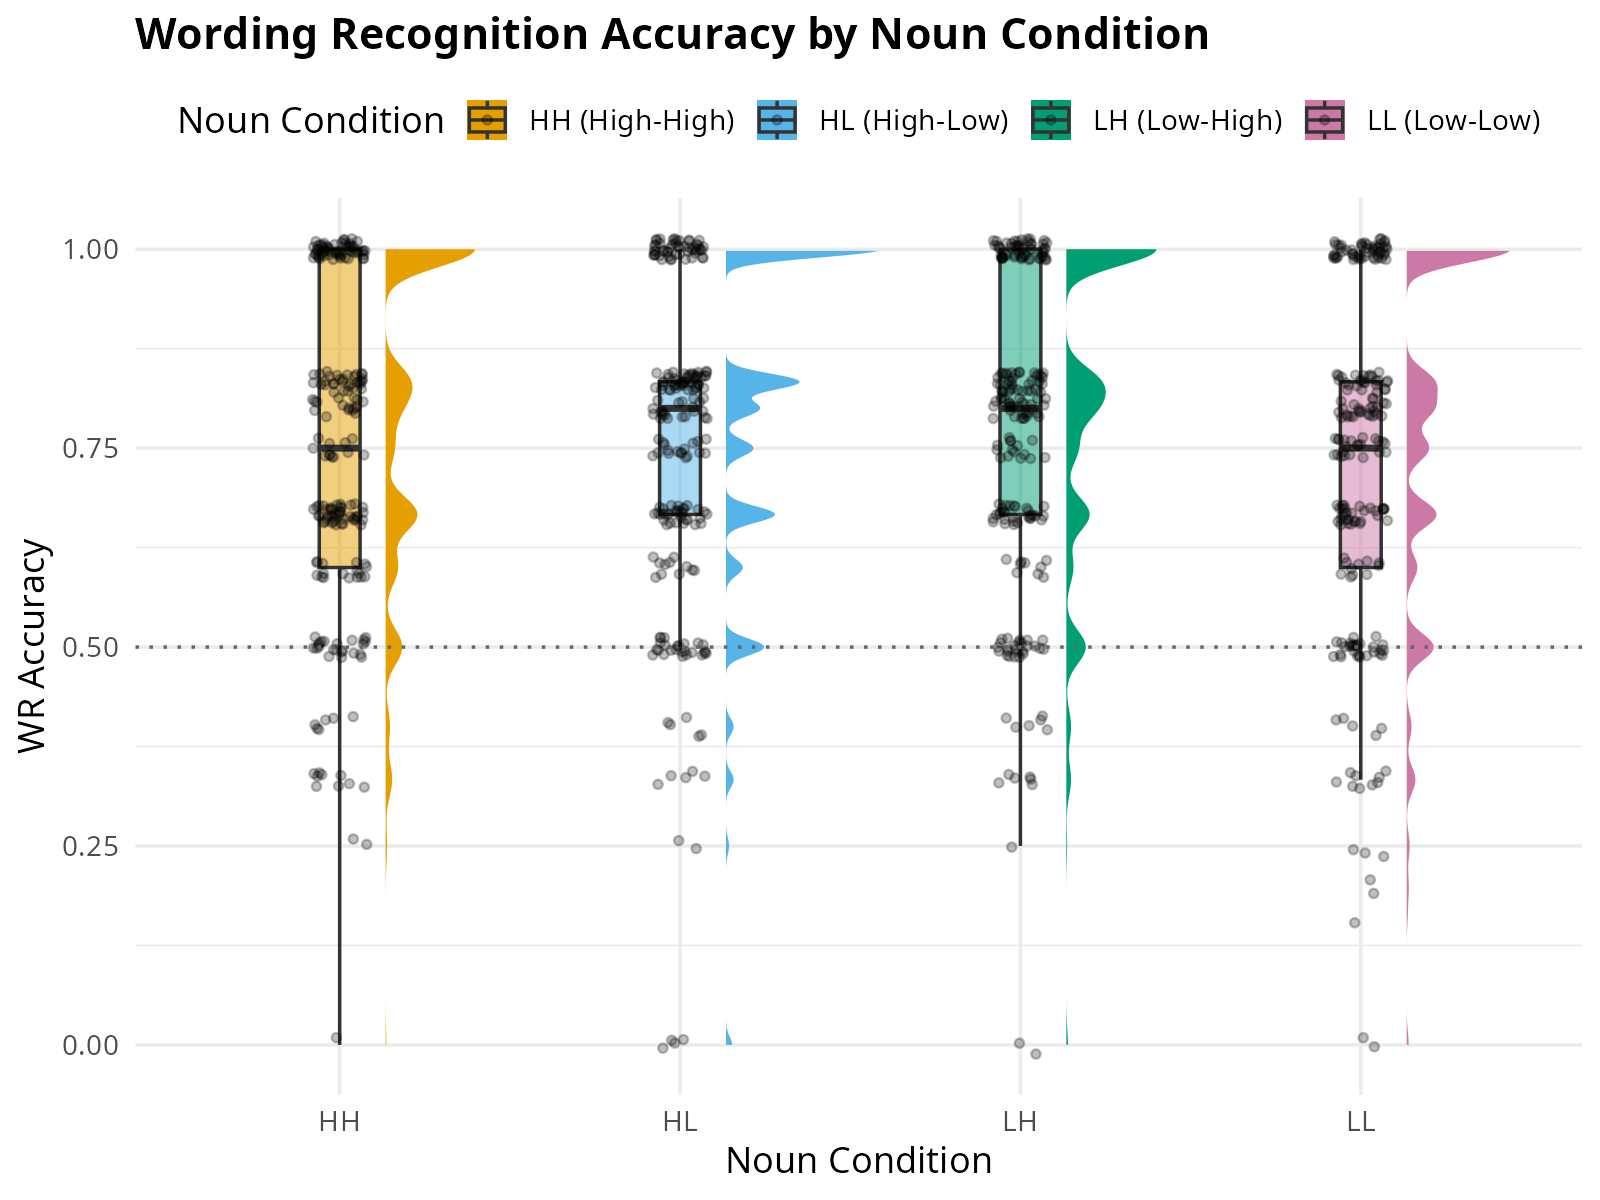
\includegraphics[width=0.85\textwidth]{plots/02_wr_acc_by_condition.png}
  \caption{WR Accuracy across noun conditions. Performance is uniformly
  high and statistically indistinguishable across all conditions.}
  \label{fig:wr_acc}
\end{figure}

Friedman's test: $\chi^2(3) = 3.34$, $p = .343$, $W = 0.010$
(small) --- non-significant at $\alpha_{\text{FW}} = .0167$. WR
performance was tested against the chance level of 0.50 (random voice
guessing) via one-sample Wilcoxon signed-rank test in each voice condition;
performance was robustly above chance in both voices ($V > 6200$,
$p < .001$, $r > .83$), confirming that participants' voice judgments
reflect genuine wording memory, not guessing. Noun imageability does
not affect syntactic retention.

% ------------------------------------------------------------
\subsection{Noun Condition $\times$ Voice Interaction (H3 \& H4)}
\label{sec:interaction}

\begin{figure}[htbp]
  \centering
  \begin{subfigure}[b]{0.48\textwidth}
    
\includegraphics[width=\textwidth]{plots/03_ir_cr_condition_x_voice.png}
    \caption{Corrected IR by Condition $\times$ Voice}
  \end{subfigure}
  \hfill
  \begin{subfigure}[b]{0.48\textwidth}
    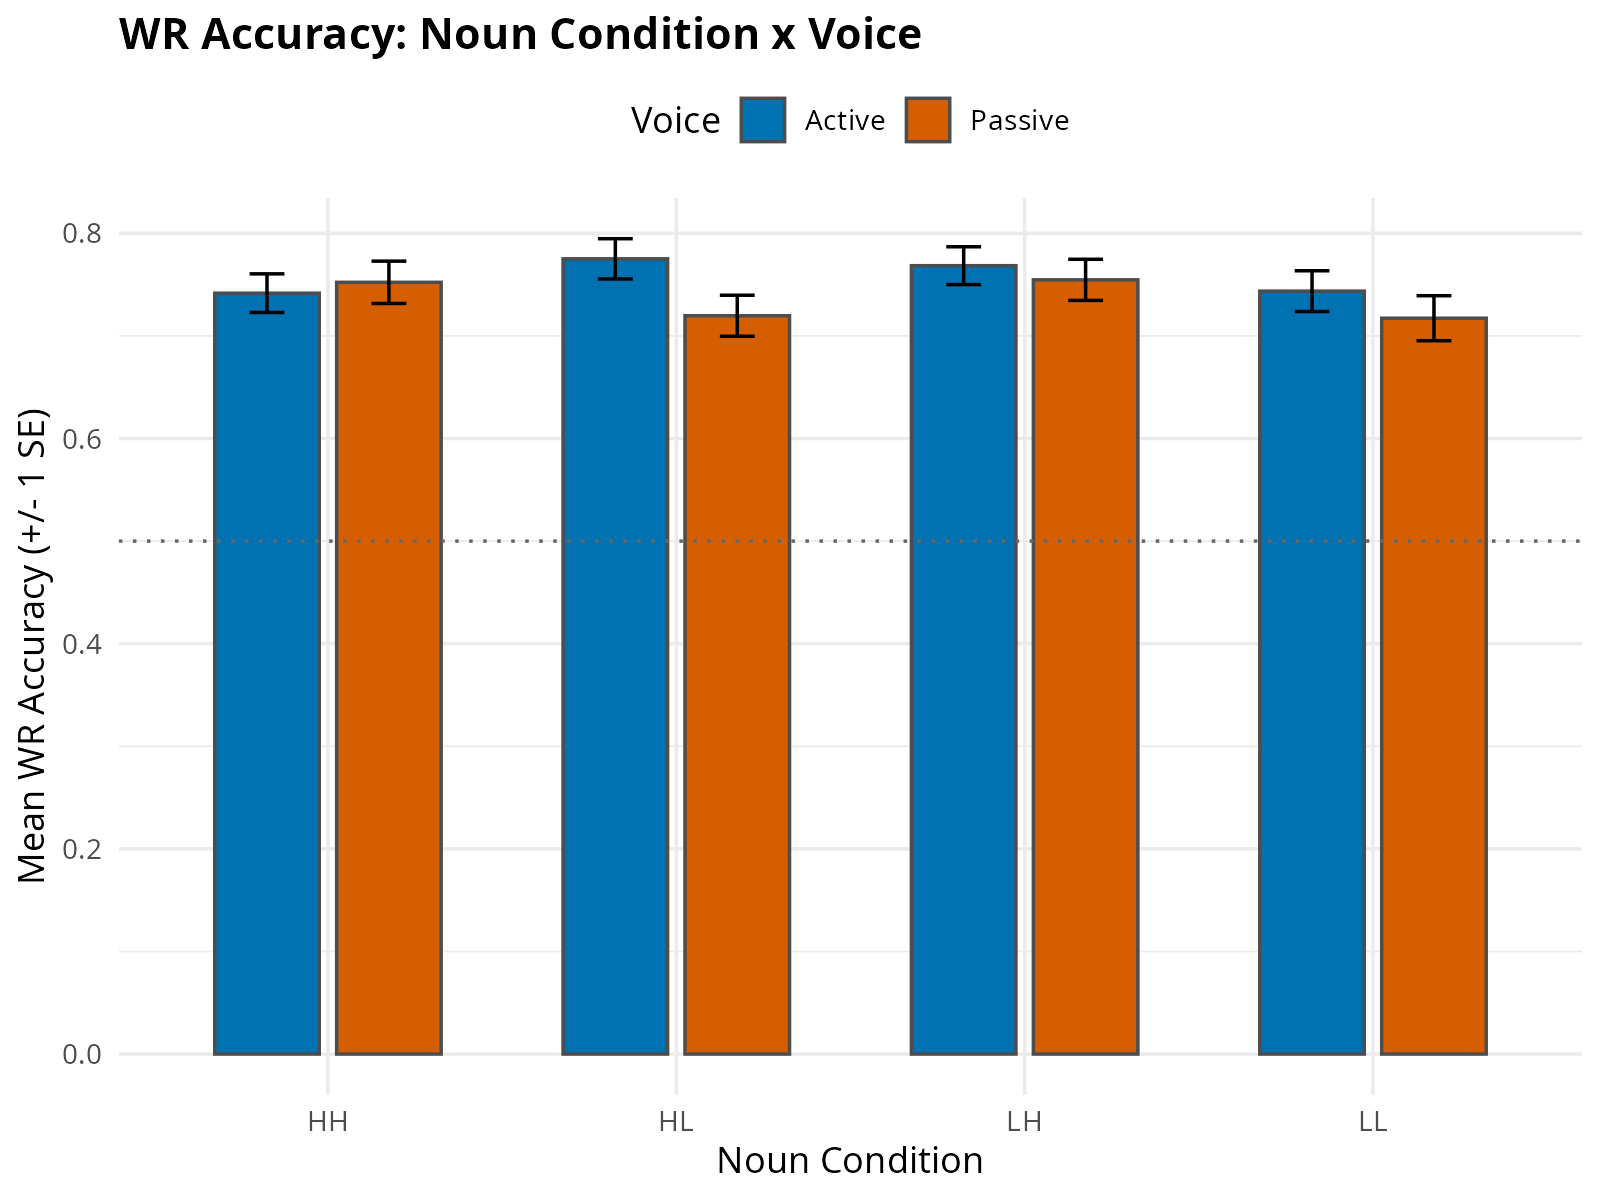
\includegraphics[width=\textwidth]{plots/04_wr_acc_condition_x_voice.png}
    \caption{WR Accuracy by Condition $\times$ Voice}
  \end{subfigure}
  \caption{Interaction plots. No systematic condition~$\times$~voice
  moderation is visible for either outcome.}
  \label{fig:interactions}
\end{figure}

SRH tests found for \textbf{Corrected IR}: noun condition main effect
($H = 11.26$, $p = .010$, $\eta^2_H = 0.013$); no voice main effect
($H = 0.76$, $p = .384$); \textbf{no interaction}
($H = 0.22$, $p = .975$, $\eta^2_H < .001$). For \textbf{WR accuracy}:
no significant effects or interaction (all $p > .23$). These results
support H4.

Paired Wilcoxon voice tests (collapsed across condition) found no
significant voice effect on Corrected IR ($V = 1916.5$, $p = .485$,
$r = .066$) or WR ($V = 3520.5$, $p = .114$, $r = .149$).

Sensitivity Friedman tests per voice level (robustness check for SRH
independence assumption): within Active voice, Corrected IR showed a
significant noun condition effect ($\chi^2(3) = 14.92$, $p = .002$,
$W = 0.045$, small); within Passive voice, the effect was likewise
significant ($\chi^2(3) = 13.67$, $p = .003$, $W = 0.041$, small).
These per-voice results confirm that the LL deficit is not confined to
one voice condition and that the SRH main effect is not an artefact of
the independence approximation.

% ------------------------------------------------------------
\subsection{IR Reaction Time}
\label{sec:rt}

\begin{figure}[htbp]
  \centering
  \begin{subfigure}[b]{0.50\textwidth}
    
\includegraphics[width=\textwidth]{plots/05_ir_rt_by_condition.png}
    \caption{IR RT by Condition}
  \end{subfigure}
  \hfill
  \begin{subfigure}[b]{0.45\textwidth}
    
\includegraphics[width=\textwidth]{plots/06_qq_ir_cr.png}
    \caption{Q-Q Plot: Corrected IR}
  \end{subfigure}
  \caption{RT distributions (left) and Q-Q plot for Corrected IR (right).
  In the Q-Q plot, deviations from the diagonal at the tails indicate
  non-normality (bounded proportions with excess skew); this confirms
  the decision to use non-parametric Friedman tests rather than
  parametric ANOVA for Corrected IR. HC3 robust SEs in the GLM further
  address the heteroscedasticity implied by these tails.}
  \label{fig:rt_qq}
\end{figure}

Friedman's test on IR RT: $\chi^2(3) = 16.53$, $p < .001$,
$W = 0.049$ (small), significant at $\alpha_{\text{FW}} = .0167$.
Post-hoc (Holm): LH vs.\ LL was the only significant pair
($p < .001$, $r = .387$). Passive LL sentences were slowest
($M = 1808$~ms vs.\ Active HL at $1664$~ms), consistent with greater
processing difficulty when both nouns are low-imageability.


% ------------------------------------------------------------
\subsection{SDT Results}

\subsubsection{Descriptive SDT Statistics}

\begin{table}[htbp]
  \centering\small
  \begin{tabular}{lcccccc}
    \toprule
    \textbf{Cond} &
    $\boldsymbol{d'_M}$ & $\boldsymbol{d'_{SD}}$ &
    $\boldsymbol{c_M}$ & $\boldsymbol{c_{SD}}$ &
    $\boldsymbol{A'_M}$ & $\boldsymbol{A'_{SD}}$ \\
    \midrule
    HH & 2.146 & 0.690 & $-$0.003 & 0.396 & 0.895 & 0.067 \\
    HL & 2.146 & 0.654 & $-$0.003 & 0.407 & 0.897 & 0.061 \\
    LH & 2.091 & 0.698 & $\phantom{-}$0.024 & 0.393 & 0.891 & 0.068 \\
    LL & 1.925 & 0.672 & $\phantom{-}$0.107 & 0.421 & 0.876 & 0.071 \\
    \bottomrule
  \end{tabular}
  \caption{SDT parameter estimates by noun condition ($N = 112$).
  $d'$ = sensitivity; $c$ = criterion ($c > 0$ = conservative);
  $A'$ = non-parametric AUC \citep{snodgrass1988}.}
  \label{tab:sdt_desc}
\end{table}

\subsubsection{Inferential Tests on $d'$ and $A'$}

Shapiro-Wilk per group confirmed normality of $d'$ ($p > .09$ all groups),
justifying RM-ANOVA. $A'$ is bounded and uses Friedman's.

\textbf{RM-ANOVA on $d'$}: Mauchly's $W = 0.961$, $p = .492$ (sphericity
assumed).
\[
  F(3, 333) = 8.47,\quad p < .001,\quad
  \text{GES} = 0.018,\quad \text{Cohen's } f = 0.134 \;(\text{small})
\]
Holm-corrected post-hoc paired $t$-tests: LL < HH ($p < .001$, $d = 0.39$),
HL ($p < .001$, $d = 0.43$), LH ($p = .010$, $d = 0.29$); HH vs.\ HL
($p = .996$) and HH vs.\ LH ($p = .768$) non-significant. Threshold
pattern confirmed.

\textbf{Friedman's on $A'$}: $\chi^2(3) = 23.50$, $p < .001$,
$W = 0.070$ (small). Post-hoc Holm: LL < HH ($r = .360$), HL ($r = .415$),
LH ($r = .256$); HH--HL, HH--LH non-significant ($p > .50$).
The $A'$ result, which makes no equal-variance assumption
\citep{snodgrass1988}, replicates the $d'$ pattern, confirming it is
not an artefact of the SDT model's distributional assumptions.

\subsubsection{Criterion ($c$) Analysis}

RM-ANOVA on $c$: $F(3, 333) = 8.47$, $p < .001$. The LL condition
shows the most positive $c$ ($M = 0.107$ vs.\
$c_{\text{HH/HL}} = -0.003$): participants required \emph{more}
subjective evidence before calling an LL sentence ``seen.''
This conservative shift occurs above and beyond the sensitivity
reduction ($d'$ is also lowest for LL), suggesting the LL deficit
comprises both a weaker imaginal trace \emph{and} a compensatory
metacognitive adjustment in decision threshold.

\subsubsection{Convergent Validity}

\begin{table}[htbp]
  \centering\small
  \begin{tabular}{lc}
    \toprule
    \textbf{Condition} & $\boldsymbol{\rho}$ \\
    \midrule
    HH & 0.981 \\ HL & 0.976 \\ LH & 0.977 \\ LL & 0.960 \\
    Overall & 0.977 \\
    \bottomrule
  \end{tabular}
  \caption{Spearman $\rho$ between $d'$ and Corrected IR ($N = 112$;
  all $p < .001$). $\rho \geq .96$ confirms Corrected IR as an adequate
  proxy for $d'$.}
  \label{tab:convergent}
\end{table}

\begin{figure}[htbp]
  \centering
  \begin{subfigure}[b]{0.32\textwidth}
    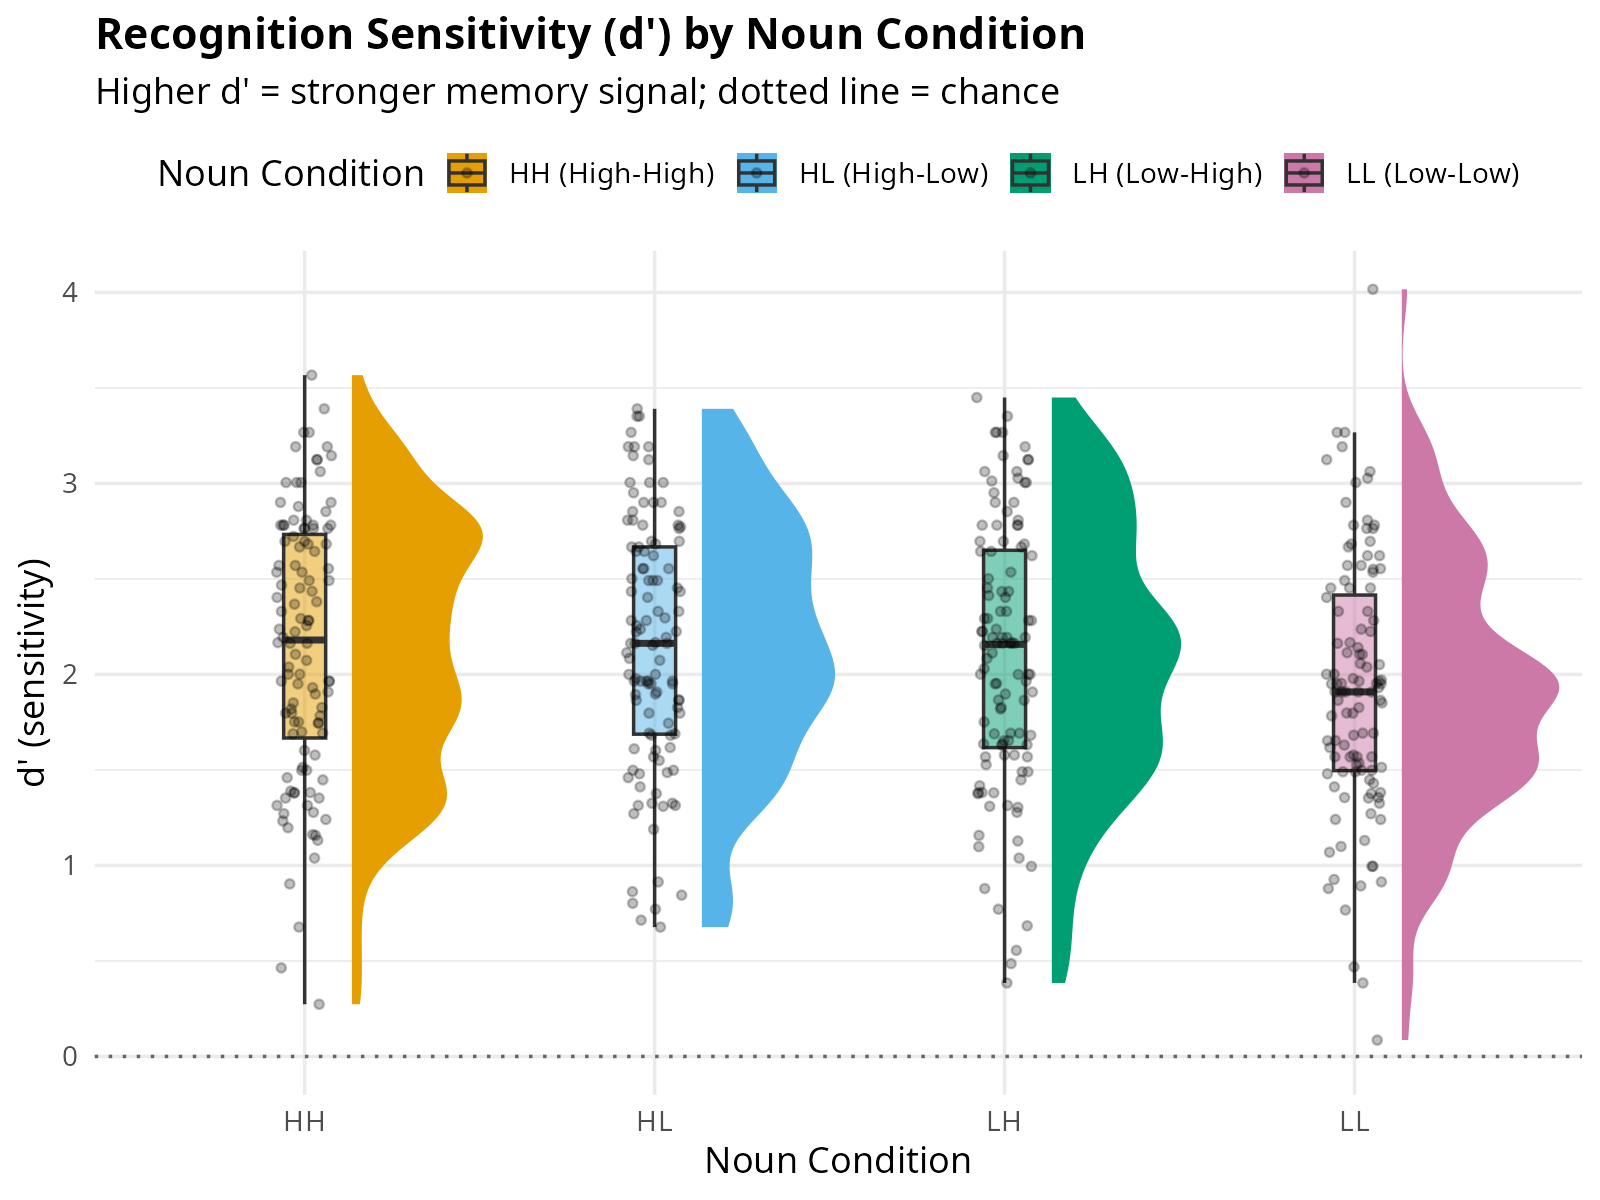
\includegraphics[width=\textwidth]{plots/sdt/01_dprime_by_condition.png}
    \caption{$d'$ by condition}
  \end{subfigure}
  \hfill
  \begin{subfigure}[b]{0.32\textwidth}
    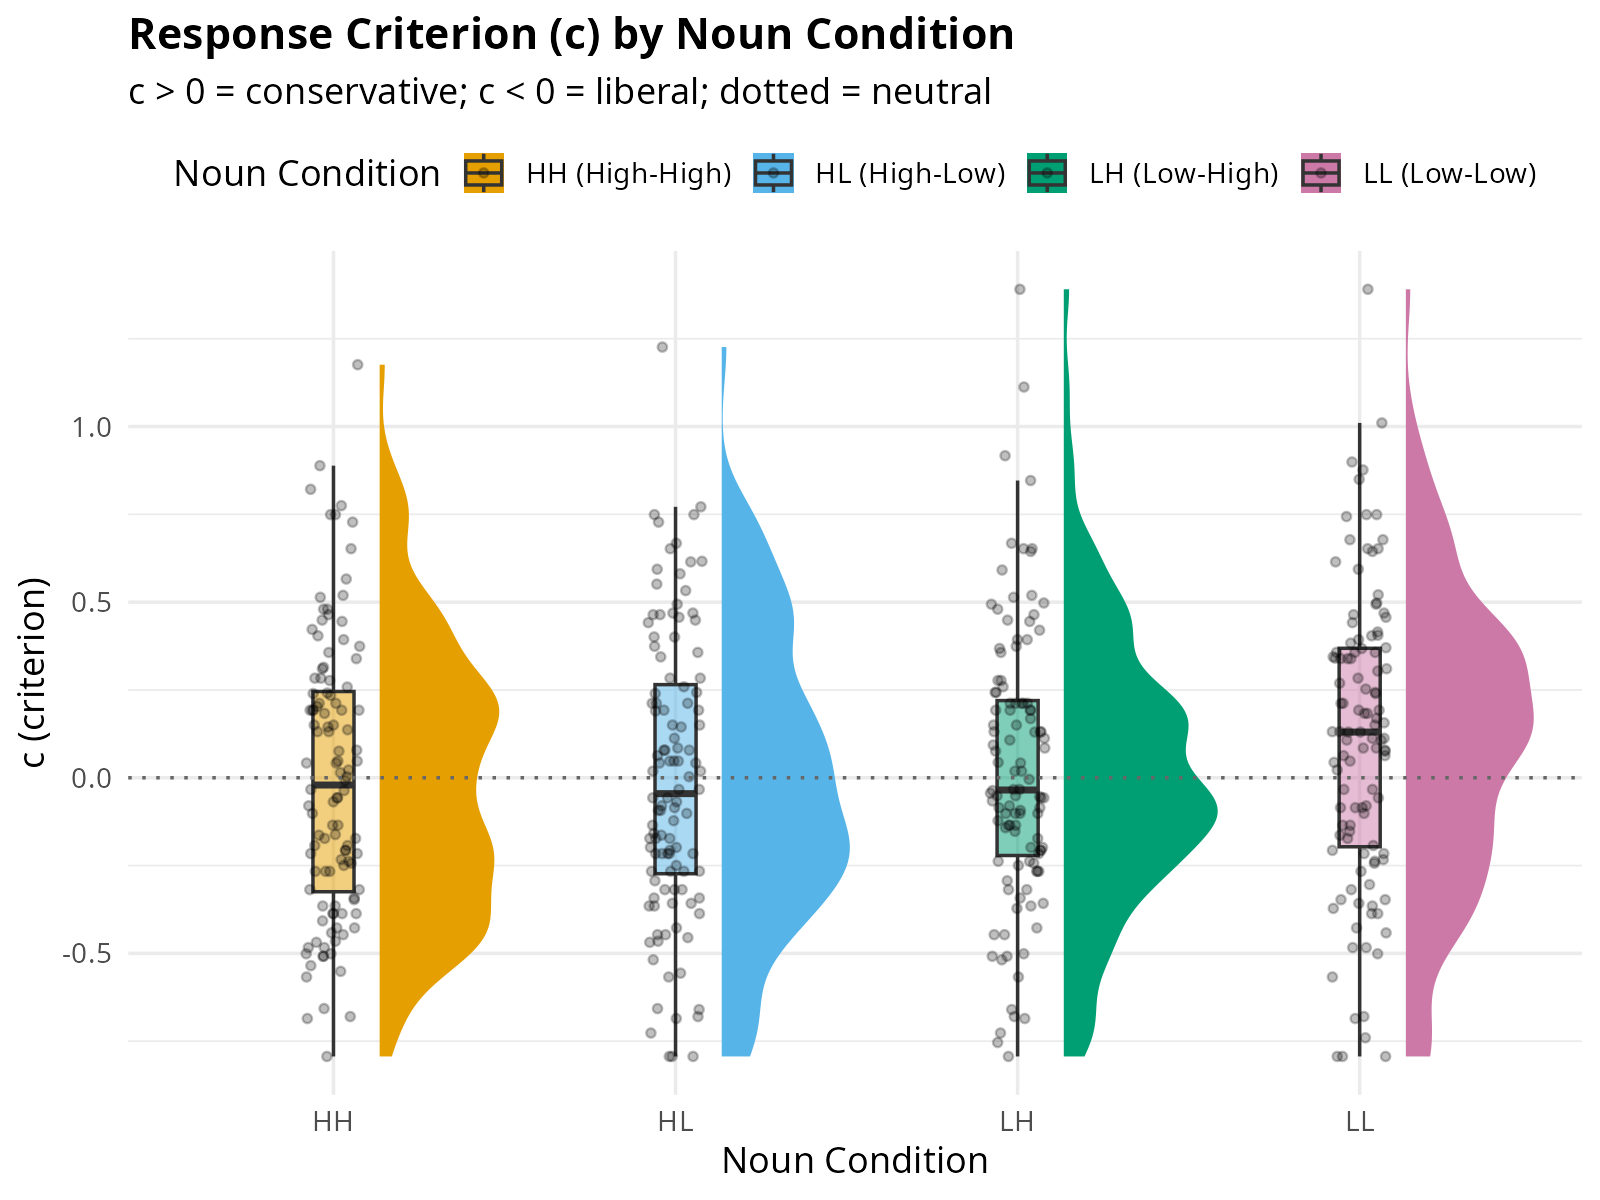
\includegraphics[width=\textwidth]{plots/sdt/02_c_by_condition.png}
    \caption{Criterion $c$}
  \end{subfigure}
  \hfill
  \begin{subfigure}[b]{0.32\textwidth}
    
\includegraphics[width=\textwidth]{plots/sdt/04_dprime_vs_corrIR.png}
    \caption{$d'$ vs.\ Corrected IR}
  \end{subfigure}
  \caption{SDT results. (a) Sensitivity lower for LL.
  (b) Criterion shifts conservatively for LL.
  (c) Near-perfect $\rho = 0.977$ between $d'$ and Corrected IR.}
  \label{fig:sdt}
\end{figure}

% ------------------------------------------------------------
\subsection{GLM Results}

\subsubsection{Corrected IR: Best Model}

Backward AIC retained:
$\text{Corrected IR} \sim \text{noun\_condition} + \text{mean\_trial\_position}$
\[
  F(4, 885) = 7.89,\quad p < .001,\quad R^2 = 0.034,\quad
  \text{Adj.} R^2 = 0.030
\]

\begin{table}[htbp]
  \centering\small
  \begin{tabular}{lccccc}
    \toprule
    \textbf{Term} & $\boldsymbol{\hat{\beta}}$ & \textbf{Robust SE} &
    $\boldsymbol{t}$ & $\boldsymbol{p}$ & \textbf{95\% CI} \\
    \midrule
    Intercept     & 0.374 & 0.070 & 5.37 & $<.001$ & [0.237, 0.512] \\
    Cond: LH      & 0.049 & 0.019 & 2.54 & .011    & [0.011, 0.088] \\
    Cond: HL      & 0.053 & 0.020 & 2.73 & .006    & [0.015, 0.092] \\
    Cond: HH      & 0.055 & 0.020 & 2.80 & .005    & [0.016, 0.094] \\
    Trial position & 0.011 & 0.003 & 3.88 & $<.001$ & [0.005, 0.017] \\
    \bottomrule
  \end{tabular}
  \caption{HC3 coefficient estimates for best Corrected IR GLM.
  Coefficients for LH, HL, HH are nearly identical (threshold pattern).
  Bayesian model comparison: BF$_{10} = 10.76$ (positive evidence).}
  \label{tab:glm_ir}
\end{table}

The near-equal $\hat{\beta}$ values for LH (0.049), HL (0.053), and HH
(0.055) confirm the threshold structure in a covariate-controlled
regression framework. Bayesian comparison: BF$_{10} = 10.76$ --- positive
evidence for noun condition predicting Corrected IR.

\subsubsection{WR Accuracy: Best Model}

Backward AIC retained: $\text{WR Accuracy} \sim \text{voice} +
\text{mean\_trial\_position}$, with noun condition eliminated from the
model (AIC penalised its inclusion as it provided no fit improvement).
\[
  F(2, 887) = 4.24,\quad p = .015,\quad R^2 = 0.010
\]

\begin{table}[htbp]
  \centering\small
  \begin{tabular}{lccccc}
    \toprule
    \textbf{Term} & $\boldsymbol{\hat{\beta}}$ & \textbf{Robust SE} &
    $\boldsymbol{t}$ & $\boldsymbol{p}$ & \textbf{95\% CI} \\
    \midrule
    Intercept      & 0.752 & 0.017 & 43.93 & $<.001$ & [0.718, 0.786] \\
    Voice: Passive & 0.019 & 0.011 &  1.75 & .081    & [$-$0.003, 0.041] \\
    Trial position & 0.011 & 0.004 &  2.57 & .010    & [0.003, 0.019] \\
    \bottomrule
  \end{tabular}
  \caption{HC3 coefficient estimates for best WR Accuracy GLM.
  Noun condition was eliminated by backward AIC.
  Bayesian comparison: BF$_{01} = 1027$ (very strong evidence against
  noun condition as a predictor of WR).}
  \label{tab:glm_wr}
\end{table}

\textbf{Noun condition was dropped} by AIC. Bayesian comparison for
noun condition: BF$_{10} = 0.001$ (BF$_{01} = 1027$) --- very strong
evidence noun condition does not predict WR.

\subsubsection{Interaction Tests (H4)}

Wald $F$-tests (HC3) confirmed no noun condition $\times$ voice interaction:
\begin{itemize}[noitemsep]
  \item Corrected IR: $F(3, 880) = 0.098$, $p = .961$;
  BF$_{01} = 97$
  \item WR Accuracy: $F(3, 880) = 0.880$, $p = .451$;
  BF$_{01} = 35$
\end{itemize}

\subsubsection{GLM Diagnostics}

\begin{figure}[htbp]
  \centering
  \begin{subfigure}[b]{0.48\textwidth}
    
\includegraphics[width=\textwidth]{plots/glm/corrected_ir_qq_residuals.png}
    \caption{Corrected IR: Q-Q residuals}
  \end{subfigure}
  \hfill
  \begin{subfigure}[b]{0.48\textwidth}
    
\includegraphics[width=\textwidth]{plots/glm/corrected_ir_residuals_vs_fitted.png}
    \caption{Residuals vs.\ Fitted}
  \end{subfigure}
  \caption{GLM diagnostic plots. HC3 robust SEs address
  heteroscedasticity; OLS point estimates remain unbiased. No
  Cook's D exceeded 1; all VIF $< 5$.}
  \label{fig:glm_diag}
\end{figure}

% ------------------------------------------------------------
\subsection{Block-Learning Results (Control Analysis)}

\subsubsection{Block Main Effect}

Friedman's test (collapsed across noun condition) on Corrected IR:
\[
  \chi^2(2) = 23.30,\quad p < .001,\quad W = 0.111 \text{ (small)}
\]
Post-hoc Holm Wilcoxon: Block 1 < Block 2 ($p < .001$, $r = .351$)
and Block 3 ($p < .001$, $r = .449$). Block 2 vs.\ 3 non-significant
($p = .166$, $r = .142$) --- learning is front-loaded and plateaus
after the first experimental block. No block effect on WR Accuracy
($\chi^2(2) = 1.42$, $p = .492$) or RT ($\chi^2(2) = 0.51$, $p = .773$).

\begin{figure}[htbp]
  \centering
  \begin{subfigure}[b]{0.48\textwidth}
    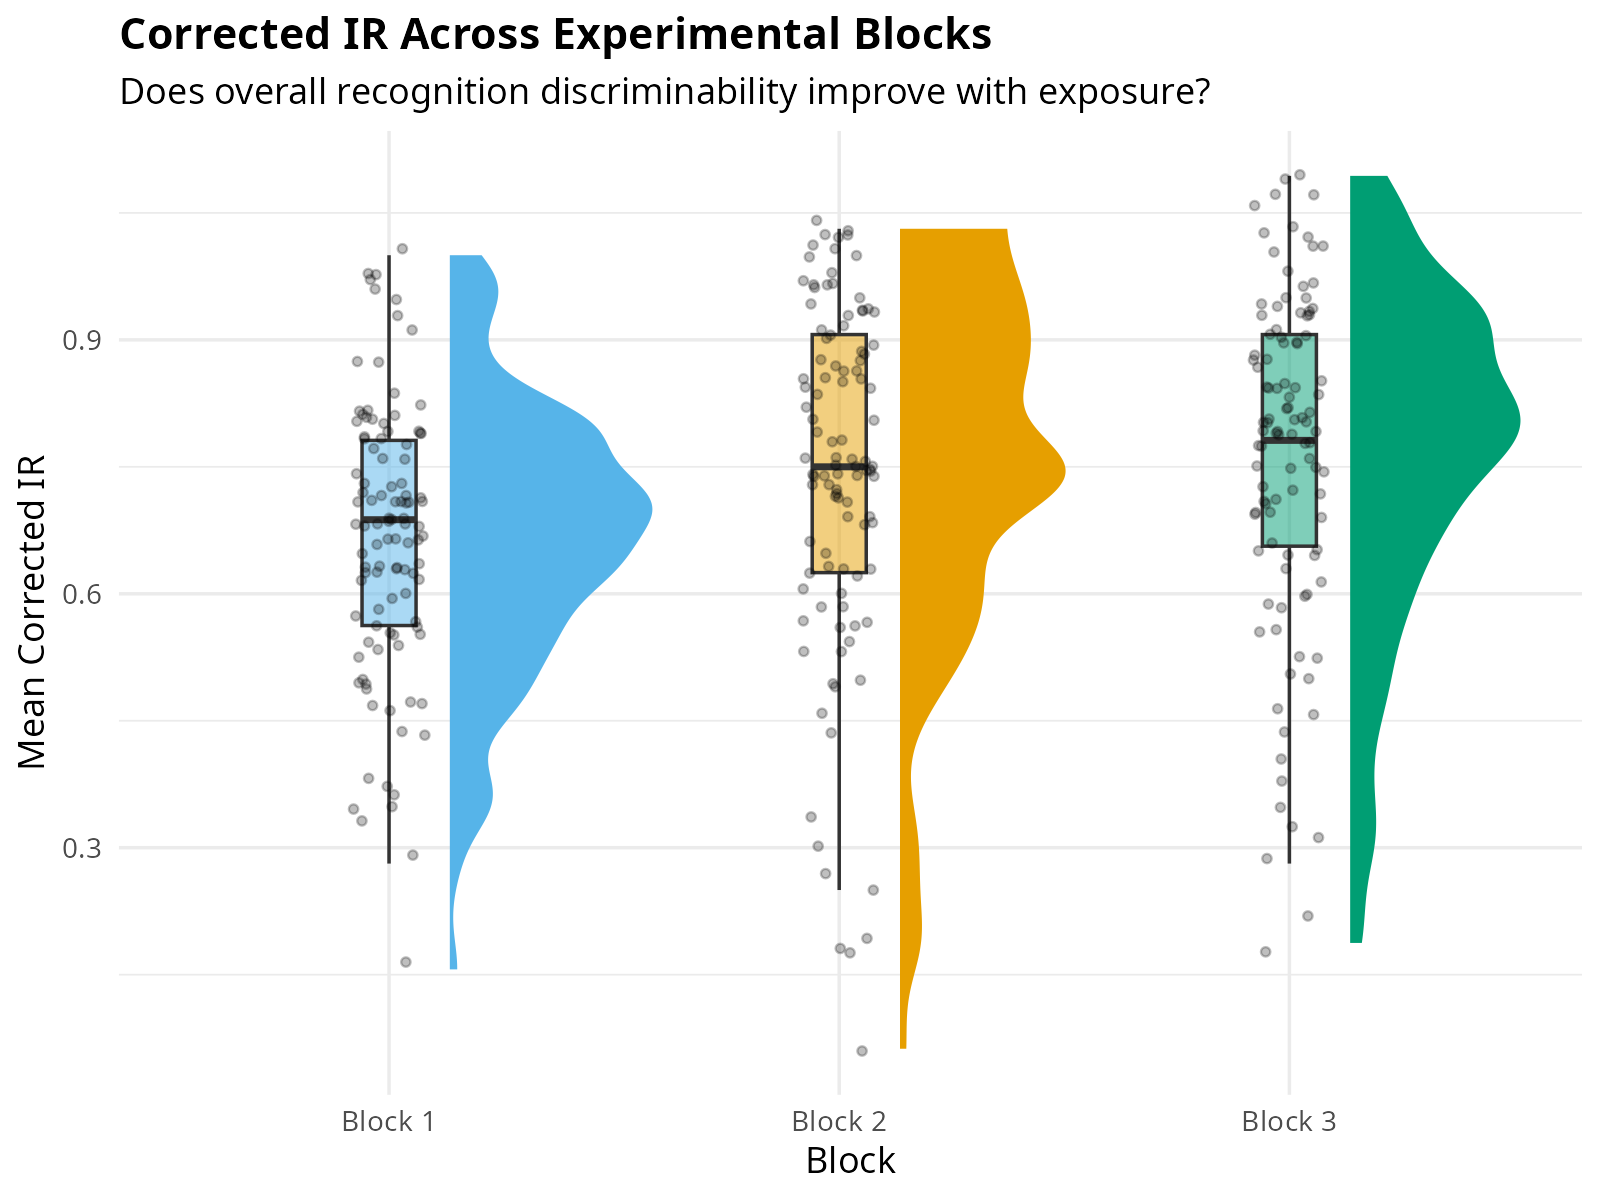
\includegraphics[width=\textwidth]{plots/block/01_ir_by_block.png}
    \caption{Corrected IR across blocks}
  \end{subfigure}
  \hfill
  \begin{subfigure}[b]{0.48\textwidth}
    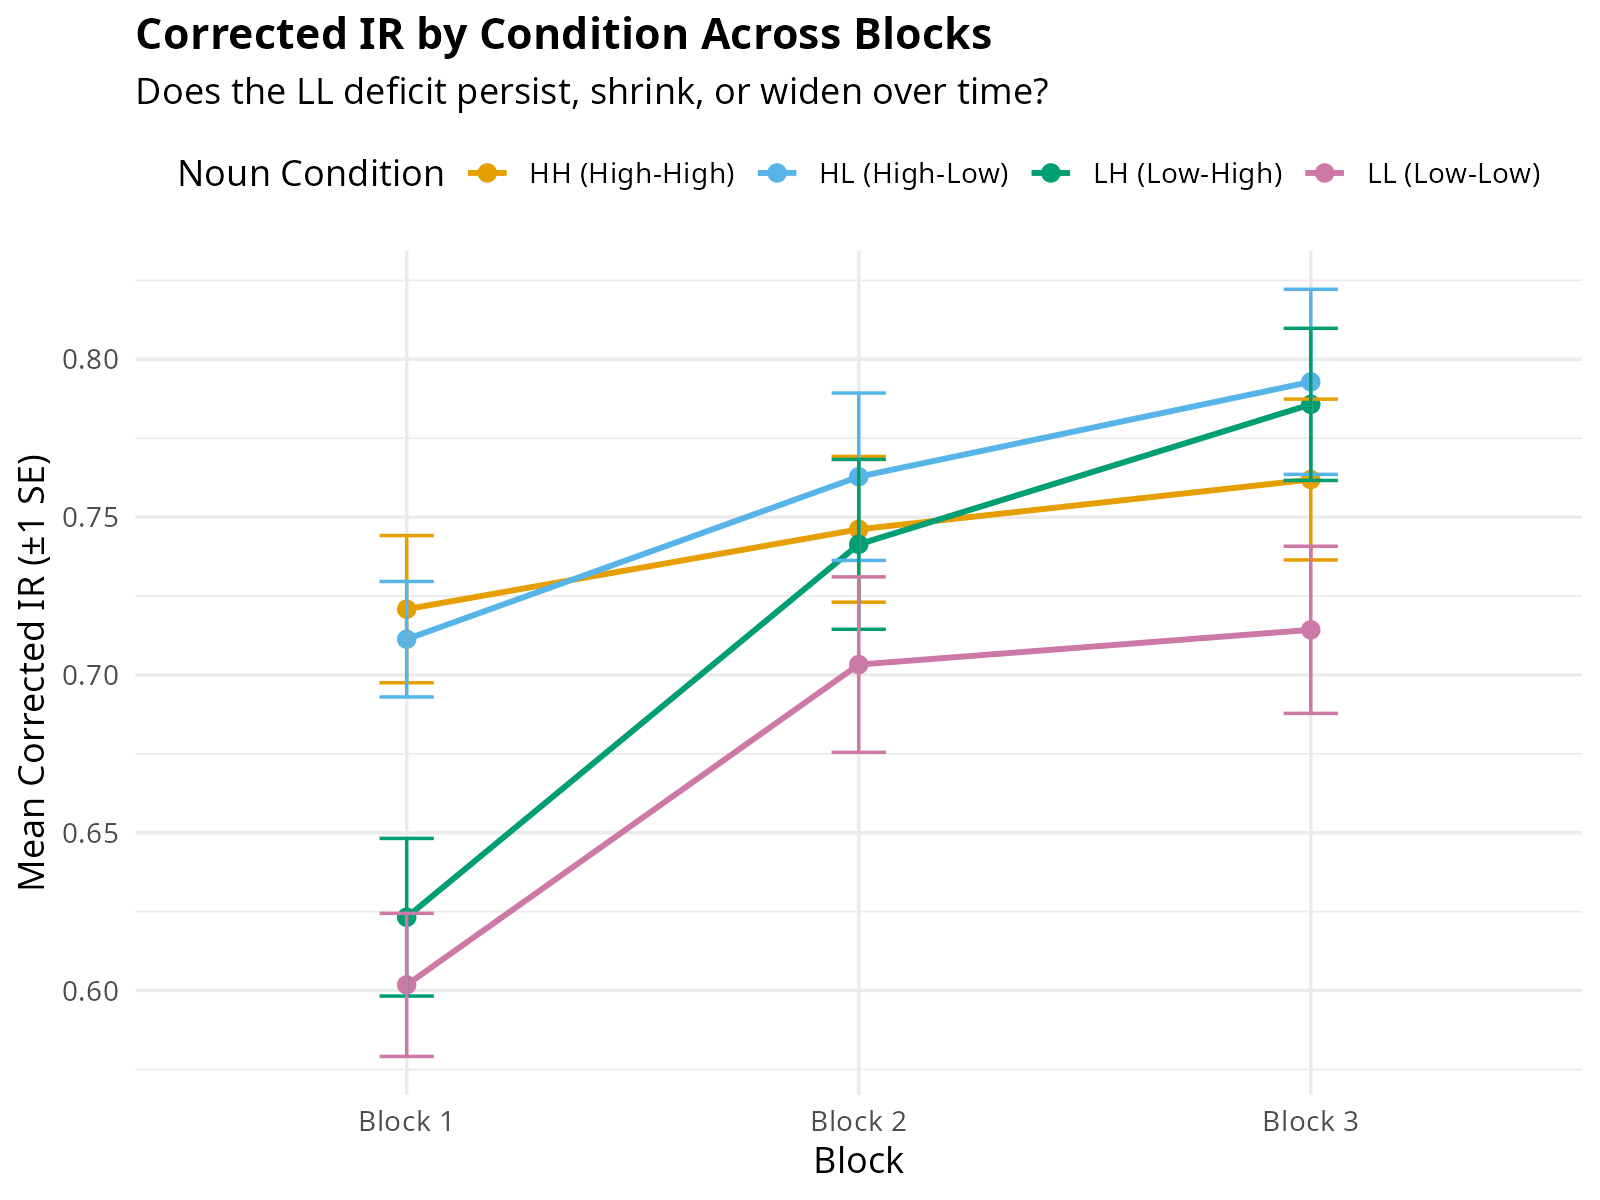
\includegraphics[width=\textwidth]{plots/block/02_ir_condition_x_block.png}
    \caption{Condition $\times$ Block}
  \end{subfigure}
  \caption{Block learning curves. IR improves Block 1 $\to$ 2 and
  plateaus. The noun condition ordering is stable across blocks;
  no condition $\times$ block interaction.}
  \label{fig:block}
\end{figure}

\subsubsection{Noun Condition Effect Within Each Block}

\begin{table}[htbp]
  \centering\small
  \begin{tabular}{lcccc}
    \toprule
    \textbf{Block} & $\boldsymbol{\chi^2(3)}$ & $\boldsymbol{p}$ &
    \textbf{Kendall's $W$} & \textbf{Significant ($\alpha_{\text{FW}}$)?} \\
    \midrule
    Block 1 & 29.0 & $<.001$ & 0.092 (small) & Yes \\
    Block 2 & 8.06 & .045    & 0.026 (small) & No ($p > .0167$)$^*$ \\
    Block 3 & 11.0 & .012    & 0.035 (small) & Yes \\
    \bottomrule
  \end{tabular}
  \caption{Per-block Friedman tests for noun condition effect on
  Corrected IR ($N = 105$, complete data across all three blocks).
  $^*$Block~2 is a descriptive trend only at the family-wise threshold.}
  \label{tab:block_omnibus}
\end{table}

\subsubsection{Condition $\times$ Block Interaction}

SRH: noun condition $H = 17.78$, $p < .001$; block $H = 51.39$,
$p < .001$; \textbf{interaction $H = 6.43$, $p = .377$}. The LL deficit
does not attenuate with repeated exposure --- it is a structural property
of the stimuli, not an artefact of early-block unfamiliarity.

% ============================================================
\section{Discussion and Conclusion}
% ============================================================

\subsection{Summary of Findings}

This study embedded the classic paradigms of \citet{begg1971} and
\citet{james1973} into a large-scale online continuous recognition task.

The \textbf{threshold model} of noun imageability is confirmed across all
four analytic frameworks. Corrected IR was impaired only when both subject
and object nouns were low-imageability (LL; Friedman's $\chi^2(3) = 22.39$,
$p < .001$). HH, HL, and LH were statistically indistinguishable (all
Holm-$p \geq .446$). This replicated in $d'$ (RM-ANOVA $F(3,333) = 8.47$,
$p < .001$) and $A'$ (Friedman's $\chi^2(3) = 23.50$, $p < .001$), was
stable across all three blocks (SRH interaction $p = .377$), and appeared
in near-equal GLM coefficients ($\hat\beta \approx 0.05$ for all three
non-LL conditions; BF$_{10} = 10.76$).

The SDT analysis adds a criterion component: LL sentences induce a
\textbf{conservative response shift} ($c_{\text{LL}} = 0.107$) above
and beyond reduced sensitivity. Participants appear aware of their
weaker memory and require stronger subjective evidence before reporting
recognition --- a metacognitive adjustment invisible to Corrected IR alone.

Noun imageability had \textbf{no effect on WR accuracy}. WR was robustly
above chance across all conditions (GLM: BF$_{01} = 1027$ for noun
condition null; Friedman's $p = .343$). Voice also had no effect on
either outcome, and no condition $\times$ voice interaction was detected
by any test.

\subsection{Theoretical Implications}

The meaning-wording dissociation replicates \citet{begg1971}'s central
finding in an online paradigm. Meaning recognition is driven by the
availability of an imagistic trace, anchored by at least one
high-imageability noun; wording recognition is independent of trace
strength, consistent with Begg's proposal that exact wording is
reconstructed at retrieval rather than stored. The absence of a voice
effect contradicts the kernel-plus-tag hypothesis of \citet{bregman1968}:
active and passive sentences are equally recognised and equally
discriminated, supporting the reconstruction account.

The threshold in recognition (vs.\ the gradient in \citet{james1973}'s
free recall) likely reflects a task difference: free recall requires
generating the sentence from memory (where every cue helps additively),
while recognition requires only that a trace reaches decision threshold
(where a single vivid anchor suffices).

\subsection{Limitations and Future Directions}

\begin{itemize}[noitemsep]
  \item \textbf{Sample size:} $N = 112$ is below the pre-registered
  target of 334; the study is underpowered for small WR and voice effects.
  At $N = 112$ and $\alpha = .017$, the design has $\approx$80\% power
  to detect Friedman effects of $W \geq 0.10$ (medium), but $\leq$50\%
  power for effects of $W < 0.05$ (small-to-negligible).
  \item \textbf{One-sided lures:} All HF lures are active-voice; passive
  $d'$ may be marginally inflated.
  \item \textbf{SRH approximation:} SRH was designed for independent
  groups; its use in a within-participants design is an approximation.
  Per-voice sensitivity Friedman tests (reported in §\ref{sec:rt})
  confirm the main finding holds within each voice level.
  \item \textbf{Future:} Reach target $N$; include passive-voice lures;
  apply Beta regression or trial-level logistic mixed-effects models;
  explore EEG correlates (N400) of the imageability effect.
\end{itemize}

% ============================================================
\section*{Team Contributions}
% ============================================================

\begin{itemize}[noitemsep]
  \item \textbf{Shreyas Deb:} End-to-end R pipeline, log parsing, FA
  rate correction, score computation, visualisations, block learning
  analysis.
  \item \textbf{Yajat Lakhanpal:} GLM pipeline (AIC selection, HC3 SEs,
  Bayesian model comparison), core non-parametric framework (Friedman,
  Wilcoxon, SRH, effect sizes).
  \item \textbf{Prasoon Dev:} Literature review and hypotheses, SDT
  analysis ($d'$, $A'$, $c$, convergent validity), Discussion and
  Theoretical Implications.
\end{itemize}

% ============================================================
\section*{Code and Data Availability}
% ============================================================

Full pipeline and source: \url{https://github.com/shrey715/sentence-memorability}

% ============================================================
{\small
\bibliographystyle{plainnat}
\bibliography{references}
}

\end{document}
